\documentclass[12pt,a4paper]{article}

\usepackage{amsmath}
\usepackage{fontspec}
\usepackage{unicode-math}
\setmainfont{Times New Roman}
\setsansfont{Calibri}
\setmathfont{Cambria Math}
\usepackage{geometry}
\geometry{top=1.35cm,bottom=1.25cm,left=1.6cm,right=1.6cm}
\usepackage{xcolor}
\usepackage{array}
\usepackage{booktabs}
\usepackage{float}
\usepackage{caption}
\captionsetup{skip=3pt,font=small,labelfont=bf}
\usepackage{fancyhdr}
\usepackage{tikz}
\usetikzlibrary{arrows.meta}
\usepackage{hyperref}
\hypersetup{colorlinks=true,linkcolor=blue!55!black,urlcolor=blue!55!black}

\setlength{\parindent}{0pt}
\setlength{\parskip}{3pt}
\setlength{\abovedisplayskip}{4pt}
\setlength{\belowdisplayskip}{4pt}
\renewcommand{\arraystretch}{1.15}
\renewcommand{\figurename}{Hình}
\renewcommand{\tablename}{Bảng}

\definecolor{criticalbar}{RGB}{211,47,47}
\definecolor{normalbar}{RGB}{63,125,190}

\pagestyle{fancy}
\fancyhf{}
\lhead{\small Quản trị dự án -- PERT}
\rhead{\small Bach Minh Quang -- 202490077}
\cfoot{\thepage}
\setlength{\headheight}{14pt}

\tikzset{
  event/.style={circle,draw=black,thick,minimum size=11mm,inner sep=0.4pt,
    font=\scriptsize\bfseries,align=center,fill=white},
  arc/.style={-{Latex[length=2.1mm]},thick,normalbar},
  criticalarc/.style={-{Latex[length=2.1mm]},very thick,criticalbar},
  dummyarc/.style={-{Latex[length=2.1mm]},dashed,thick,gray!65!black},
  arclabel/.style={font=\scriptsize\bfseries,fill=white,inner sep=1pt}
}

\begin{document}

\begin{center}
  {\large\bfseries ĐẠI HỌC BÁCH KHOA HÀ NỘI}\\[0.5pt]
  {\bfseries Trường Công nghệ Thông tin và Truyền thông}\\[4pt]
  {\Large\bfseries BÀI TẬP PERT}\\[1pt]
  {\small Bach Minh Quang \quad MSSV: 202490077 \quad Hà Nội, 09/2026}
\end{center}
\vspace{-3pt}
\hrule
\vspace{6pt}

\begin{table}[H]\centering
\caption{Dữ liệu công việc (MSSV 202490077)}
\small
\begin{tabular}{cccccc}
\toprule
\textbf{CV} & \textbf{Trình tự} & \textbf{$d$} & \textbf{CV} & \textbf{Trình tự} & \textbf{$d$}\\
\midrule
$X$ & Từ đầu & 3 & $U$ & Từ đầu & 12\\
$Y$ & Sau $X$ & 4 & $T$ & Sau $V,U$ & 5\\
$Z$ & Từ đầu & 3 & $S$ & Từ đầu & 4\\
$V$ & Sau $Y,Z$ & 3 & $W$ & Sau $T,S$ & 7\\
\bottomrule
\end{tabular}
\end{table}

\paragraph{a. Sơ đồ PERT \hfill {\normalfont\small (3 điểm)}}
Mạng AOA. Mũi đỏ: công việc găng. Mũi xanh: không găng. Nét đứt: việc giả ($d=0$).
Trong đỉnh: số hiệu sự kiện và $t_s/t_m$.

\begin{figure}[H]\centering
\resizebox{0.97\linewidth}{!}{%
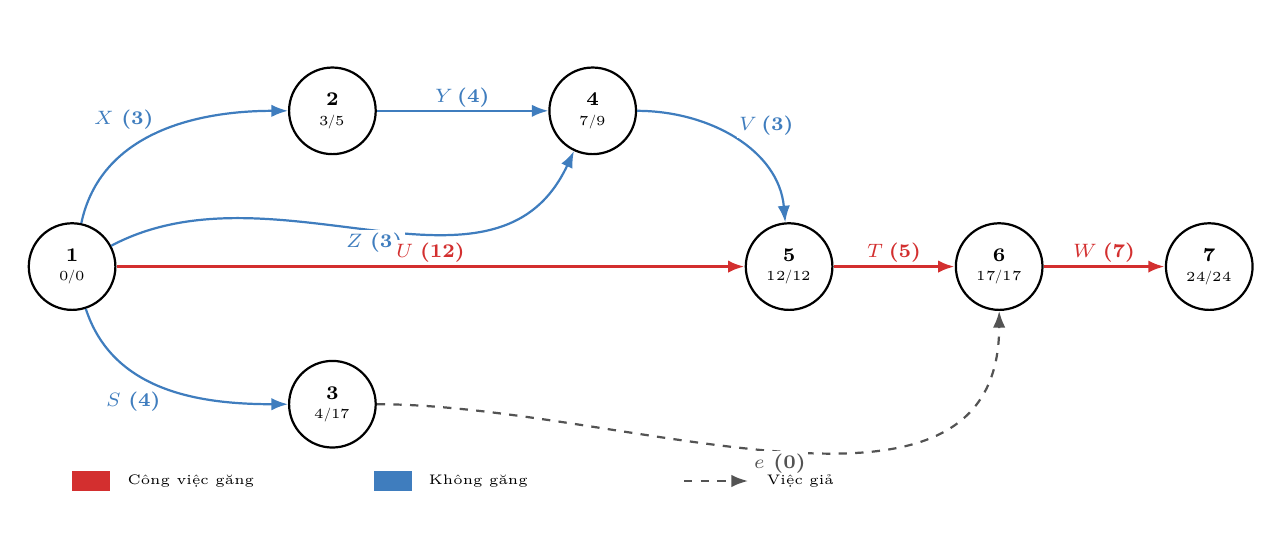
\begin{tikzpicture}[x=1.16cm,y=0.92cm]
  \node[event] (p1) at (0.00,1.55) {1\\[-1pt]{\tiny\normalfont $0/0$}};
  \node[event] (p2) at (2.85,3.70) {2\\[-1pt]{\tiny\normalfont $3/5$}};
  \node[event] (p3) at (2.85,-0.35) {3\\[-1pt]{\tiny\normalfont $4/17$}};
  \node[event] (p4) at (5.70,3.70) {4\\[-1pt]{\tiny\normalfont $7/9$}};
  \node[event] (p5) at (7.85,1.55) {5\\[-1pt]{\tiny\normalfont $12/12$}};
  \node[event] (p6) at (10.15,1.55) {6\\[-1pt]{\tiny\normalfont $17/17$}};
  \node[event] (p7) at (12.45,1.55) {7\\[-1pt]{\tiny\normalfont $24/24$}};

  \draw[arc] (p1) to[out=78,in=180] node[arclabel,above left] {$X$ (3)} (p2);
  \draw[arc] (p2) -- node[arclabel,above] {$Y$ (4)} (p4);
  \draw[arc] (p1) to[out=28,in=245] node[arclabel,below] {$Z$ (3)} (p4);
  \draw[arc] (p4) to[out=0,in=95] node[arclabel,above right] {$V$ (3)} (p5);
  \draw[criticalarc] (p1) -- node[arclabel,above] {$U$ (12)} (p5);
  \draw[criticalarc] (p5) -- node[arclabel,above] {$T$ (5)} (p6);
  \draw[arc] (p1) to[out=-72,in=180] node[arclabel,below left] {$S$ (4)} (p3);
  \draw[dummyarc] (p3) to[out=0,in=-90] node[arclabel,below] {$e$ (0)} (p6);
  \draw[criticalarc] (p6) -- node[arclabel,above] {$W$ (7)} (p7);

  \fill[criticalbar] (0.0,-1.55) rectangle +(0.42,0.28);
  \node[anchor=west,font=\tiny] at (0.50,-1.41) {Công việc găng};
  \fill[normalbar] (3.3,-1.55) rectangle +(0.42,0.28);
  \node[anchor=west,font=\tiny] at (3.80,-1.41) {Không găng};
  \draw[dummyarc] (6.7,-1.41) -- +(0.70,0);
  \node[anchor=west,font=\tiny] at (7.50,-1.41) {Việc giả};
\end{tikzpicture}}
\caption{Mạng PERT. Đường găng $U-T-W$.}
\end{figure}

\paragraph{b. Chỉ tiêu các sự kiện (đỉnh) \hfill {\normalfont\small (2 điểm)}}
Tính tiến: $t_s(j)=\max_{i\rightarrow j}\{t_s(i)+d_{ij}\}$, $t_s(1)=0$.
Tính lùi: $t_m(i)=\min_{i\rightarrow j}\{t_m(j)-d_{ij}\}$, $t_m(7)=t_s(7)$.
Dự trữ đỉnh $R(i)=t_m(i)-t_s(i)$; đỉnh găng khi $R=0$.

{\small
\textbf{Tiến:}
$t_s(1)=0$,
$t_s(2)=3$,
$t_s(3)=4$,
$t_s(4)=\max(3+4,0+3)=7$,
$t_s(5)=\max(7+3,0+12)=12$,
$t_s(6)=\max(12+5,4+0)=17$,
$t_s(7)=17+7=24$.
\\
\textbf{Lùi:}
$t_m(7)=24$,
$t_m(6)=17$,
$t_m(5)=12$,
$t_m(4)=9$,
$t_m(3)=17$,
$t_m(2)=5$,
$t_m(1)=\min(2,6,13,0)=0$.
}

\begin{table}[H]\centering
\caption{Thời điểm sớm, muộn và dự trữ các sự kiện}
\begin{tabular}{c|ccccccc}
\toprule
Sự kiện $i$ & 1 & 2 & 3 & 4 & 5 & 6 & 7\\
\midrule
$t_s(i)$ & 0 & 3 & 4 & 7 & 12 & 17 & 24\\
$t_m(i)$ & 0 & 5 & 17 & 9 & 12 & 17 & 24\\
$R(i)$   & 0 & 2 & 13 & 2 & 0 & 0 & 0\\
\bottomrule
\end{tabular}
\end{table}

Đỉnh găng: $1,5,6,7$.

\paragraph{c. Thời gian sớm nhất hoàn thành dự án \hfill {\normalfont\small (0,25 điểm)}}
$T=t_s(7)=t_m(7)=\mathbf{24}$ ngày.
Đối chiếu: $U{+}T{+}W=12{+}5{+}7=24$;
$X{+}Y{+}V{+}T{+}W=22$;
$Z{+}V{+}T{+}W=18$;
$S{+}W=11$.

\paragraph{d. Đường găng \hfill {\normalfont\small (0,75 điểm)}}
Công việc găng khi $TF_{ij}=t_m(j)-t_s(i)-d_{ij}=0$: $U(1{\rightarrow}5)$, $T(5{\rightarrow}6)$, $W(6{\rightarrow}7)$.
\[
  \boxed{U-T-W\qquad (12+5+7=24\ \text{ngày})}
\]

\end{document}
